\section*{Lezione 2}
\addcontentsline{toc}{section}{Lezione 2}


Supponiamo di avere una sorgente S che emette un simbolo ogni colpo di clock.
Questo simbolo subisce una codifica di sorgente (per compattare la rappresentazione dell'informazione) e successivamente, prima di immettere nel canale, bisogna effettuare una codifica di canale.
Il canale è rumoroso per definizione, quindi bisogna aggiungere al simbolo delle cifre di controllo.
Il messaggio quindi sarà composto da \textit{m} bit di messaggio e \textit{k} bit di controllo, il totale farà \textit{n}.

\begin{figure}[h]
	\centering
	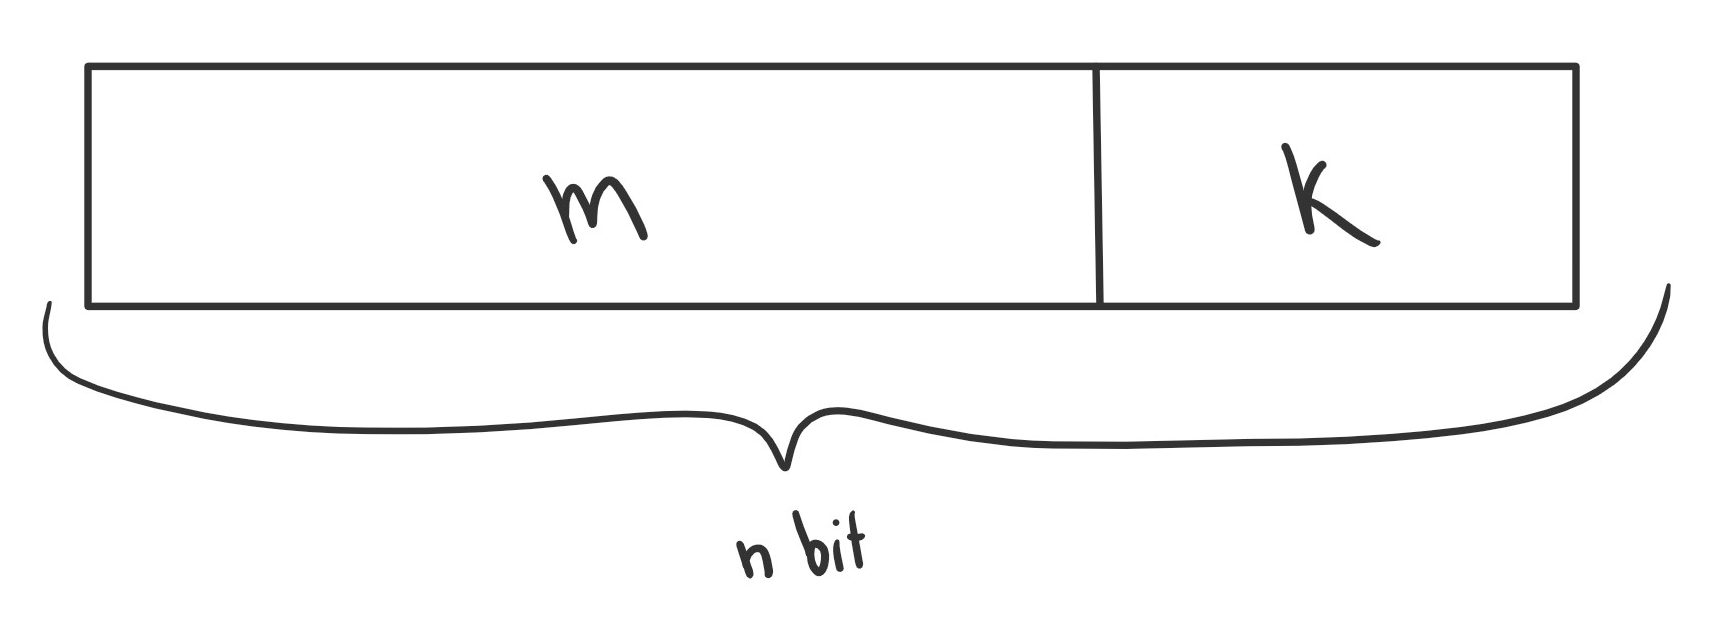
\includegraphics[width=\linewidth]{immagini/img1}
	\caption{Struttura messaggio da inserire nel canale}
\end{figure}

Le cifre di controllo servono ad aumentare la ridondanza del messaggio, in questo modo per il ricevente sarà più facile capire se ci sono stati errori.\\
La \textbf{ridondanza} serve per capire meglio il messaggio (esempio, se togli una lettera dall'alfabeto italiano le parole si capiscono comunque, però con quella lettera è più veloce capire).

\subsection*{Controllo di parità singolo - Codifica di canale}
\addcontentsline{toc}{subsection}{Codifica di canale}

Si aggiunge una cifra alla fine del messaggio.
Ci sono due tipi di parità:
\begin{itemize}
	\item Parità pari: il bit equivale a 1 se il numero di 1 nel messaggio è dispari (in questo modo si arriva ad avere un numero pari di 1).
	il bit equivale a 0 se il numero di 1 nel messaggio è pari (il numero è già pari, quindi non aggiungo altri 1)
	\item Parità dispari: stesso ragionamento ma al contrario.
\end{itemize}

Di base useremo la parità pari, hanno stesse proprietà (in certi casi si usa quella dispari, es. mando pacchetto di zeri su linea con 0 volt).

Per il calcolo del bit di parità si usa una funzione di parità:
\begin{equation}
y = \textrm{Parity(}x_1, x_2, ..., x_n\textrm{)} = x_1 \oplus x_2 \oplus ... \oplus x_n
\end{equation}
In questo modo quando il ricevente legge il messaggio, controlla che il numero di 1 sia pari.
Se non lo è, allora c'è stato un errore singolo.

La stessa funzione può essere vista come:

\begin{equation}
y = \textrm{Parity(}x_1, x_2, ..., x_n\textrm{)} = x_1 + x_2 + ... + x_n \; \text{mod} \; 2
\end{equation}

Questo è utile quando si vuole trattare 0 e 1 con i loro significati numerici.
Isomorfismo fra queste due forme:

\begin{figure}[h]
	\centering
	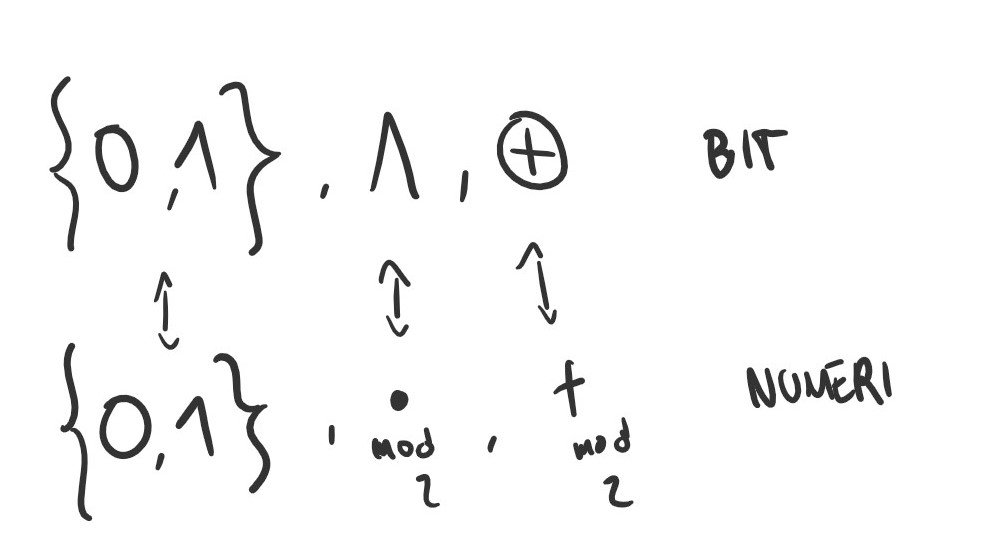
\includegraphics[width=0.6\linewidth]{immagini/img2}
	\caption{Isomorfismo bit/numeri}
\end{figure}

Per fare il calcolo della funzione Parity(\textit{x}) di solito si basa l'hardware (visto che è un operazione molto diffusa, ogni hardware ha supporto per questo tipo di calcoli).
In caso l'hardware supporti solo ad esempio lo xor fra due soli bit, posso scomporre in questo modo ed effettuarne uno ad uno:

\begin{equation}
x_1 \oplus x_2 \oplus x_3 \oplus x_4 \oplus x_5 = (x_1 \oplus x_2) \oplus (x_3\oplus x_4) \oplus (x_5 \oplus 0)
\end{equation}
\begin{center}
n.b.\\
$x \oplus 0 = x$\\
$x \oplus 1 = \lnot x$
\end{center}

Si potrebbe anche utilizzare un automa a stati finiti per modellare il problema:

\begin{figure}[h]
	\centering
	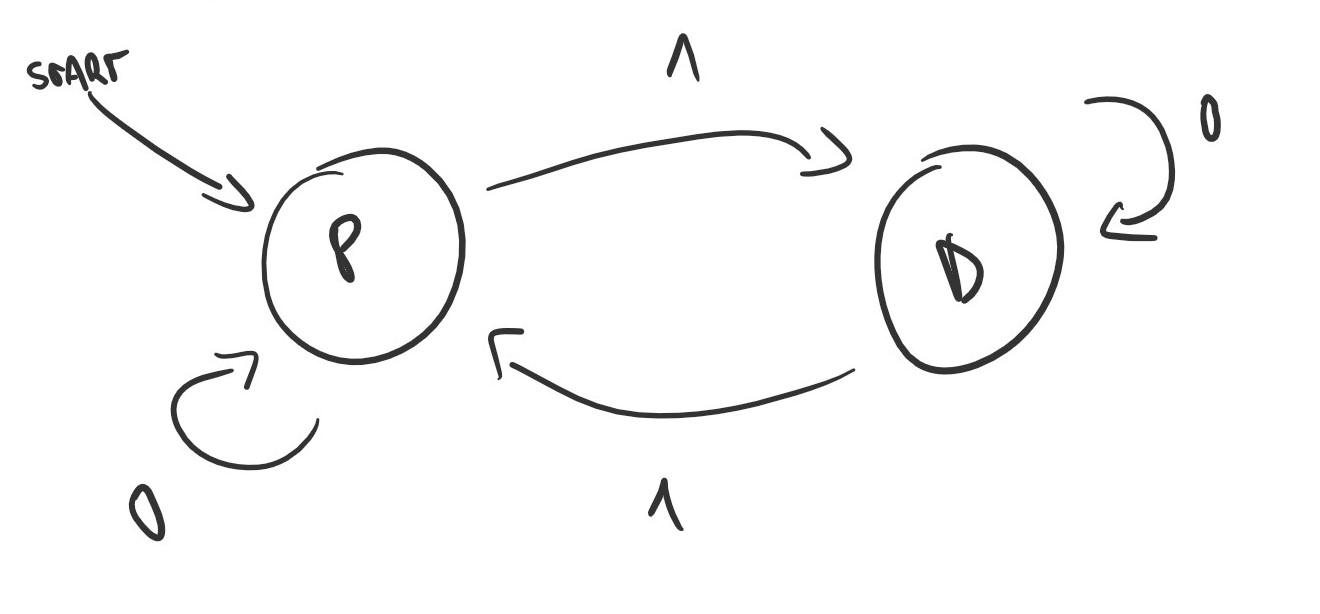
\includegraphics[width=0.6\linewidth]{immagini/img3}
	\caption{Automa a stati finiti per il calcolo pari/dispari}
\end{figure}

\subsection*{Ridondanza}
\addcontentsline{toc}{subsection}{Ridondanza}

Con ridondanza intendiamo, data la Figura 1, questo rapporto:
\begin{equation}
R = \frac{\text{numero di cifre totali}}{\text{numero di cifre di controllo}} = \frac{n}{m} \geq 1
\end{equation}
Con \textit{k = 0} la ridondanza vale 1, e praticamente stiamo inserendo il messaggio senza bit di parità.\\
In altri termini si dice che:
\begin{equation}
R = 1 + \text{eccesso di ridondanza}
\end{equation}
\begin{equation*}
R = 1 + \frac{k}{m}
\end{equation*}
Quando si definisce un metodo per il controllo degli errori, si cerca di avere un eccesso di ridondanza minore possibile (meno bit si usano nel canale, meno errori avverranno; ma in generale meglio ottimizzare).

Quanto vale la ridondanza nel caso del controlli di parità?

\begin{equation}
R_{\text{parity}} = \frac{n}{n-1} = \frac{(n-1)+1}{n-1} = 1 + \frac{1}{n-1}
\end{equation}

Quindi l'eccesso di ridondanza è $\frac{1}{n-1}$.

Ovviamente, osservando come l'eccesso di ridondanza sia uguale a $\frac{k}{m}$, a parità di \textit{m}, il numero di bit del messaggio, il modo di ridurre al minimo la ridondanza è quello di minimizzare il numeratore, quindi la \textit{k}.
In gergo si dice che ogni cifra di controllo dovrà \textit{coprire} il maggior numero di bit di messaggio possibile, per avere una bassa ridondanza.


\subsection*{Canale - modelli di rumore}
\addcontentsline{toc}{subsection}{Canali - Modelli di rumore}

Il canale più semplice e facile da gestire è il \textbf{rumore bianco}, definito da queste proprietà:
\begin{itemize}
	\item La probabilità che avvenga un errore in ciascuna posizione è uguale a \textit{p} per ogni bit.
	Di conseguenza la probabilità che la trasmissione avvenga in modo corretto è $1-p$.
	\item Il fatto che avvenga un errore in posizione \textit{i} non influisce sulle altre probabilità, quindi si parla di eventi statisticamente indipendenti (condizione che rende poco realistico il rumore bianco, es. sbalzo di corrente).
\end{itemize}

Nell'intero pacchetto, qual è la probabilita di avere \textit{k} errori, dato $0 \leq k \leq n$?
Ragioniamo prima sul valore di \textit{p}
\begin{itemize}
	\item $p = 0$? No, impossibile che in un canale ci sia completa assenza di errore (qualunque supporto io utilizzi, col tempo si deteriora).
	\item $p = 1$? No, se no basta una porta not al ricevitore per avere tutti i bit corretti (come prima).
	\item $p > \frac{1}{2}$? Potrebbe aver senso, però se ho un canale che sbaglia più della metà delle volte, basta una porta not per ridurre questa quantità fino a una quantità minore di $\frac{1}{2}$ 
	\item $p = \frac{1}{2}$? Così ottengo un generatore di numeri casuali perfetto in quanto ogni bit viene trasformato in modo casuale in 0 o in 1 (cosa impossibile).
\end{itemize}

Possiamo concludere dicendo che \textit{p} è sempre $0 < p < \frac{1}{2}$.

Tornando alla domanda di prima, quanto è la probabilità di avere \textit{k} errori?\\
Partiamo dalla probabilità di avere 1 errore, esso può avvenire in una posizione qualsiasi.
Essendo eventi stocastici e statisticamente indipendenti, la probabilità di un errore è uguale a
\begin{equation}
p(\text{1 errore}) = p(E_1 \lor E_2 \lor ... \lor E_n)
\end{equation}
Con $E_k$ s'intende l'evento che avvenga un errore in posizione \textit{k}.\\
Quanto è la probabilità che avvenga un errore \textit{solo} nella posizione 2?
\begin{equation}
p(\text{errore in pos 2}) = (1-p) \; p \; (1-p)(1-p) \; ... \; (1-p)
\end{equation}
\begin{equation*}
= p \; (1-p)(1-p) \; ... \; (1-p)
\end{equation*}
\begin{equation*}
= p \; (1-p)^{n-1}
\end{equation*}

Ovviamente al posto della seconda posizione, questa regola vale per ogni posizione (proprietà commutativa della moltiplicazione).

Quindi la probabilità di avere un solo errore:
\begin{equation}
p(\text{1 errore}) = p(\text{errore in pos 1}) + p(\text{errore in pos 2}) + \; ... \; + p(\text{errore in pos n})
\end{equation}
\begin{equation*}
= np(1-p)^{n-1}
\end{equation*}

E la probabilità di ottenere 2 errori?\\
Vediamo prima la probabilità di ottenere 2 errori in 2 posizioni fissate:
\begin{equation}
p(\text{errori in pos 1 e 2}) = p \cdot p \; (1-p)(1-p) \; ... \; (1-p)
\end{equation}
\begin{equation*}
= p^2 \; (1-p)(1-p) \; ... \; (1-p)
\end{equation*}
\begin{equation*}
= p^2 \; (1-p)^{n-2}
\end{equation*}

Come posso creare le combinazioni di queste posizioni?

\begin{equation}
\binom{n}{2} = \frac{n(n-1)}{2}
\end{equation}

Quindi questo è il numero di modi in cui posso disporre gli errori nel pacchetto

Da qui, la probabilità di ottenere 2 errori è:

\begin{equation}
p(\text{2 errori}) = \binom{n}{2} p^2 (1-p)^{n-2}
\end{equation}

Riprendendo la probabilità di avere un errore, essa si può riscrivere come:

\begin{equation}
p(\text{1 errore}) = \binom{n}{1} p^1 (1-p)^{n-1}
\end{equation}

Ora, generalizzando, si può rispondere alla domanda: qual è la probabilità che si verifichino \textit{k} errori in un messaggio di \textit{n} bit (errori disposti in qualsiasi posizione all'interno del pacchetto)?

\begin{equation}
p(\text{k errori}) = \binom{n}{k} p^k (1-p)^{n-k} \; \; \; \; \; \; \text{per} \; 0 \geq k \geq n
\end{equation}

Vediamo ora come si comporta la funzione $p(\text{errori})$ dati un \textit{n} e un \textit{p} fissati.
\begin{figure}[h]
	\centering
	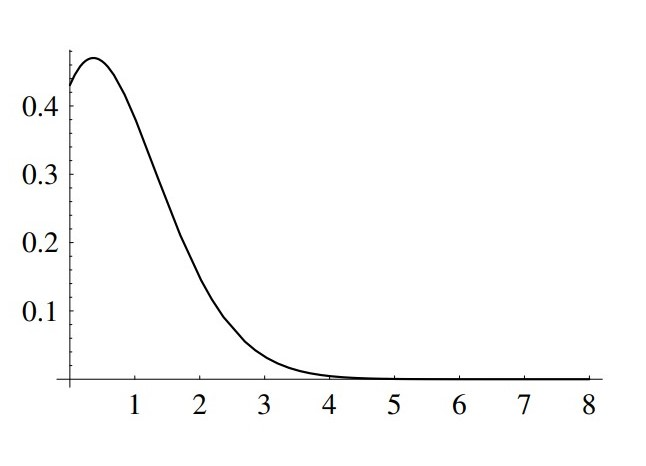
\includegraphics[width=0.6\linewidth]{immagini/img4}
	\caption{Grafico di $\binom{n}{k}p^k (1-p)^{n-k}$ con $n=8$ e $p=0.1$}
\end{figure}

Ma se all'interno del pacchetto avviene un numero pari di errori? Il controllo di parità fallisce in quanto il numero di 1 è pari (numero pari di 1 iniziale + numero pari di errori = numero pari di 1).
Viceversa se il numero di errori è dispari, allora il controllo di parità se ne accorge.

Quanto è la probabilità che il controllo di parità fallisca? In altri termini: quanto è la probabilità che avvenga un numero pari di errori?

Procediamo per passi; recuperiamo la probabilità di commettere un errore dall'equazione (13):

\begin{equation}
p(\text{1 errore}) = \binom{n}{1} p^1 (1-p)^{n-1}
\end{equation}
\begin{equation*}
= np(1-p)^{n-1}
\end{equation*}

Ricordiamo un'approssimazione sfruttando le serie di Taylor:

\begin{equation}
(1+x)^{\alpha} \approx 1 + \alpha x \; \; \; \; \; \; \text{per} \; |x| < 1
\end{equation}

Possiamo considerare \textit{n} come molto minore di $\frac{1}{p}$, quindi scrivere:

\begin{equation}
np(1-p)^{n-1}
\end{equation}
\begin{equation*}
\approx np[1-p(n-1)] 
\end{equation*}
\begin{equation*}
= np[1-p(n-1)]
\end{equation*}
\begin{equation*}
= np[1-np+p]
\end{equation*}
\begin{equation*}
= np[1-np+p]
\end{equation*}
\begin{equation*}
np-n^2p^2+np^2 
\end{equation*}

Ora trascuriamo i termini con $p^2$ in quanto essendo minore di 1, dominerà \textit{p}; quindi

\begin{equation}
p(\text{1 errore})\approx np
\end{equation}
\begin{equation*}
= \binom{n}{1}p
\end{equation*}

Per due errori:

\begin{equation}
p(\text{2 errori})\approx np \binom{n}{2}p^2
\end{equation}
\begin{equation*}
= \binom{n}{2}p^2
\end{equation*}

Generalizzando per \textit{k} errori:

\begin{equation}
p(\text{\textit{k} errori})\approx np \binom{n}{k}p^k
\end{equation}

Quindi, tornando al problema di prima, dobbiamo fare un'osservazione:

\begin{equation}
	\sum_{k=0}^{n} \binom{n}{k} p^k(1-p)^{n-k} = 1
\end{equation}

Se sommo tutte le probabilità, fare zero errori, fare un errore, fare due errori ecc. ovviamente ho come somma 1 (evento stocastico).

Sfrutto questa proprietà:
\begin{equation}
(a+b)^n = \sum_{k=0}^{n} \binom{n}{k} a^kb^{n-k}
\end{equation}

\bigskip
\bigskip

... 
Lezione 02 parte 3 min 33 +-
...

\bigskip
\bigskip
Quindi la probabilità che il controllo di parità fallisca è
\begin{equation}
p(\text{controllo parità fallisce}) = \frac{1 + (1-2p)^n}{2}-(1-p)^n
\end{equation}

\subsection*{Burst di errori}
\addcontentsline{toc}{subsection}{Burst di errori}

Gli errori nella realtà avvengono in maniera non indipendente, di solito avvengono errori su sequenze di bit adiacenti.
Definiamo \textit{L} come lunghezza del \textbf{burst} di errori.

La parola \texttt{ciao} in ASCII è rappresentata in questo modo:
\begin{center}
	\texttt{C} = 1000011\\
	\texttt{I} = 1001001\\
	\texttt{A} = 1000001\\
	\texttt{O} = 1001111
\end{center}

... fine lezione 02 parte 3








